\chapter{Constraint Verification with RWFM Labels}
\label{ch:label}
Information flow policies require some data related to objects and subjects to enforce any security protocol on them.
Each object and subject needs to specify information related to permission like who can read, who can write etc. Label or security class is a way to represent this information. Information flow policies add some prerequisite condition with each operation on objects based on labels of objects and subject.
\section{RWFM label \cite{rwfm}}
Reader Writer Flow Model label has three tuple (s,R,W)
the first s is a subject, R is a set of subjects allowed to read object, W is a set of subjects allowed to write and subjects who influenced this object so far. 
\subsection{Secure Information Flow}
All information flow security models follow property of lattice because, for secure flow, information must flow from less secure class or label to more secure class or label, any reverse flow is a violation of security.
So each information flow model redefines $\leqslant$ operator to check validity of flow.\\
\textbf{Label1} = ($s_1,R_1,W_2$), \textbf{Label2} = ($s_2,R_2,W_2$)\\
information can flow from Label1 to Label2 if and only if $R_1 \supseteq R_2$ and $W_1 \subseteq W_2$.  
\subsection{Definition of Join and Meet operations \cite{rwfm}}
\textbf{Join:} Label1 $\oplus$ Label2 = $(s_3,R_1 \cap R_2, W_1 \cup W_2)$\\
\hspace*{0.6cm}\textbf{Meet:} Label1 $\otimes$ Label2 = $(s_3,R_1 \cup R_2, W_1 \cap W_2)$
\subsection{Create, Read and Write operations on objects with RWFM label \cite{rwfm}}
If a subject $s^{(s,R_1,W_1)}$ creates object o, o will be assigned a default label derived from subject is $(s,R_1,W_1 \cup \{s\})$.
Clearance of subject s is assumed (s,$R_s$,$W_s$), clearance is used to set an upper bound on labels of a subject.\\
\textbf{Read:} A subject $s^{(s_1,R_1,W_1)}$ can read object $o^{(s_2,R_2,W_2)}$ if and only if s $\in$ $R_2$ and ($R_1$ $\cap$ $R_2$) $\supseteq$ $R_s$ $\land$ ($W_1$ $\cup$ $W_2$) $\subseteq$ $W_s$. after read operation label of subject s changes into $(s_1,R_1 \cap R_2, W_1 \cup W_2)$\\
 \textbf{Write:} A subject $s^{(s_1,R_1,W_1)}$ can read object $o^{(s_2,R_2,W_2)}$ if and only if s $\in$ $W_2$ and $R_1 \supseteq R_2 \land W_1 \subseteq$ W2. 
\section{Constraint Verification}
First of all constraint checker script processes inputs and populate data structures. Inputs are two files, one has all constraints generated by our constraint generator script, other has labels of each object provided by user. Figure \ref{fig:script2} shows modules of script2 with flow of control. After preprocessing of given constraints and labels, script provides answer to following queries.\\ 
\begin{figure*}[ht]
	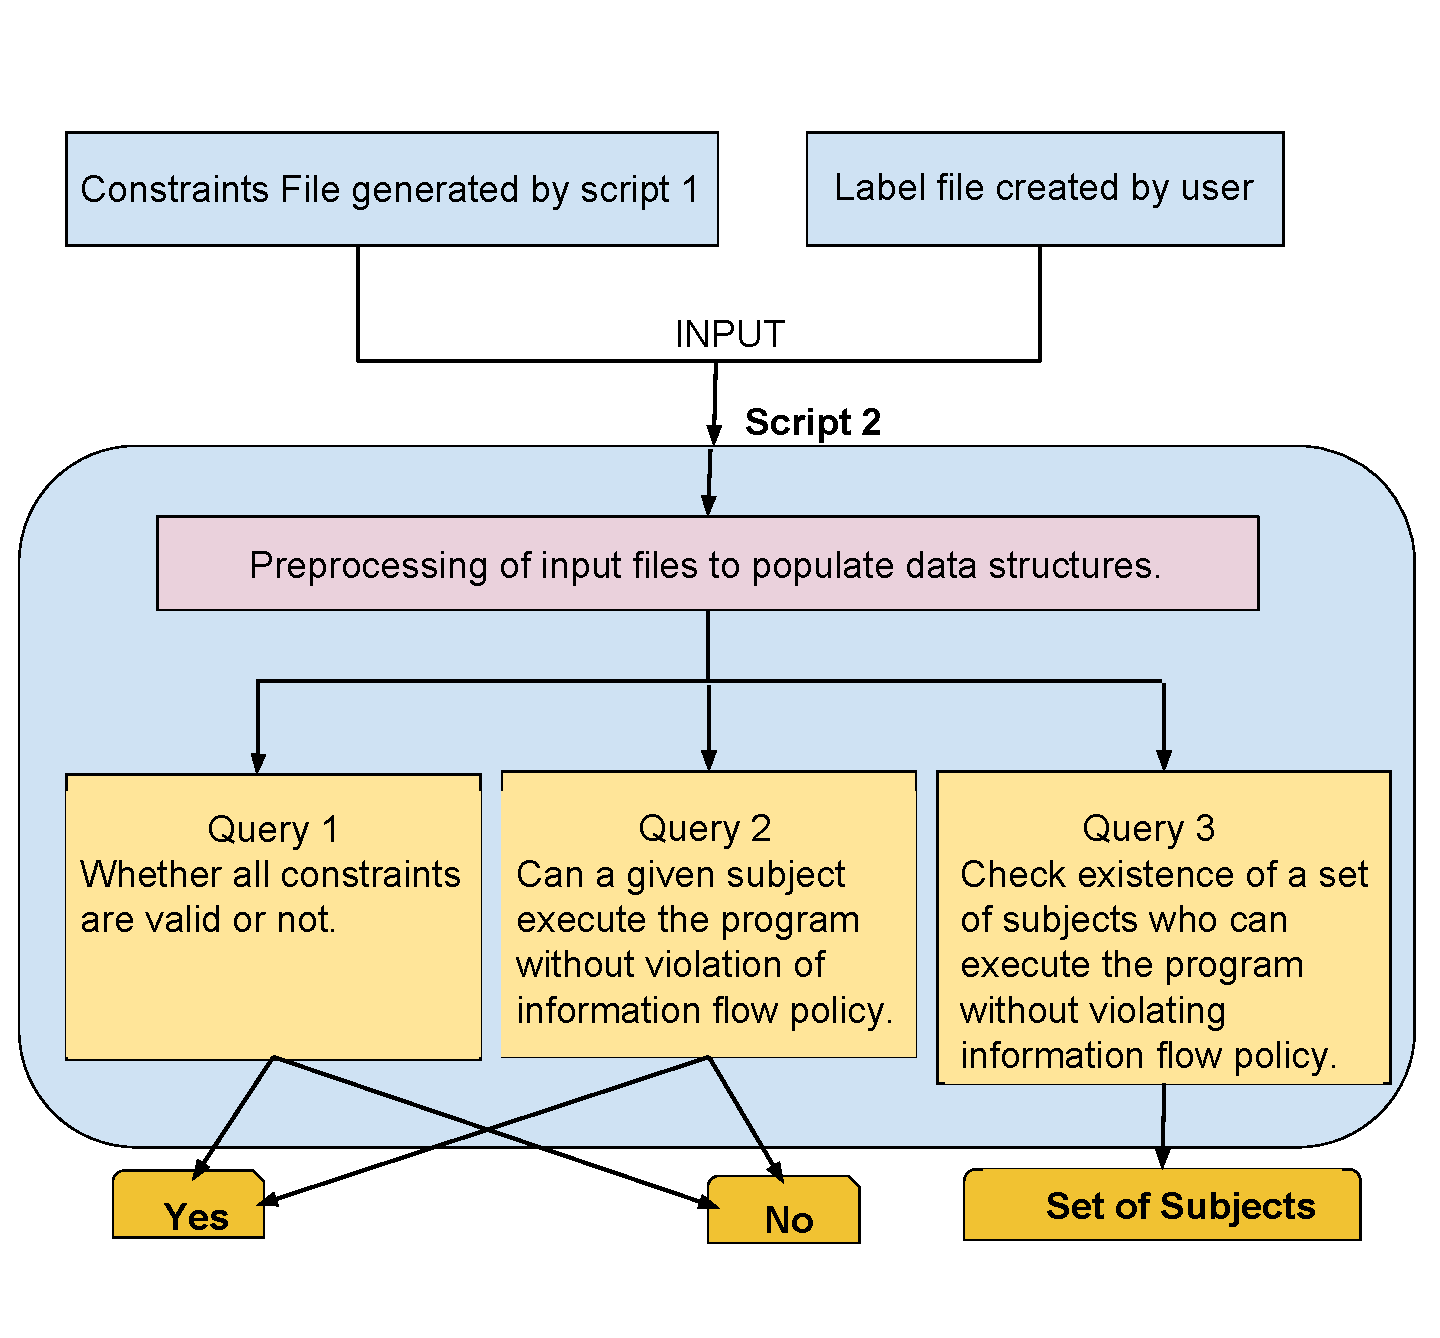
\includegraphics[width=0.7\textwidth]{constraint_checker.pdf}
	\centering
	\caption{Block diagram of script2}
	\label{fig:script2}
\end{figure*}
\begin{enumerate}
	\item{\textbf{Whether all constraints are valid or not.}\\
		Constraint format in input file : \dud{x} $\le$ \dud {y}.\\
		Format of RWFM labels : label(x) ($s_1,R_1,W_1$)\\
		\hspace*{4.5cm}label(y) ($s_2,R_2,W_2$)\\
		Definition of $\leqslant_{RWFM}$ operator in RWFM model  : label(x) $\leqslant_{RWFM}$ label(y) if only if $R_1 \supseteq R_2$ and $ W_1 \subseteq W_2 $ \hspace*{1cm}\cite{rwfm}\\
		Script reads all constraints from input file one by one then converts all objects involved in constraint into RWFM label and  checks whether they follow $\leqslant_{RWFM}$, if any constraint fails to follow $\leqslant_{RWFM}$ then returns false otherwise true.
		} 
	\item{\textbf{Can a given subject execute the program without violation of information flow policy.}\\
		\begin{figure*}
			\centering
			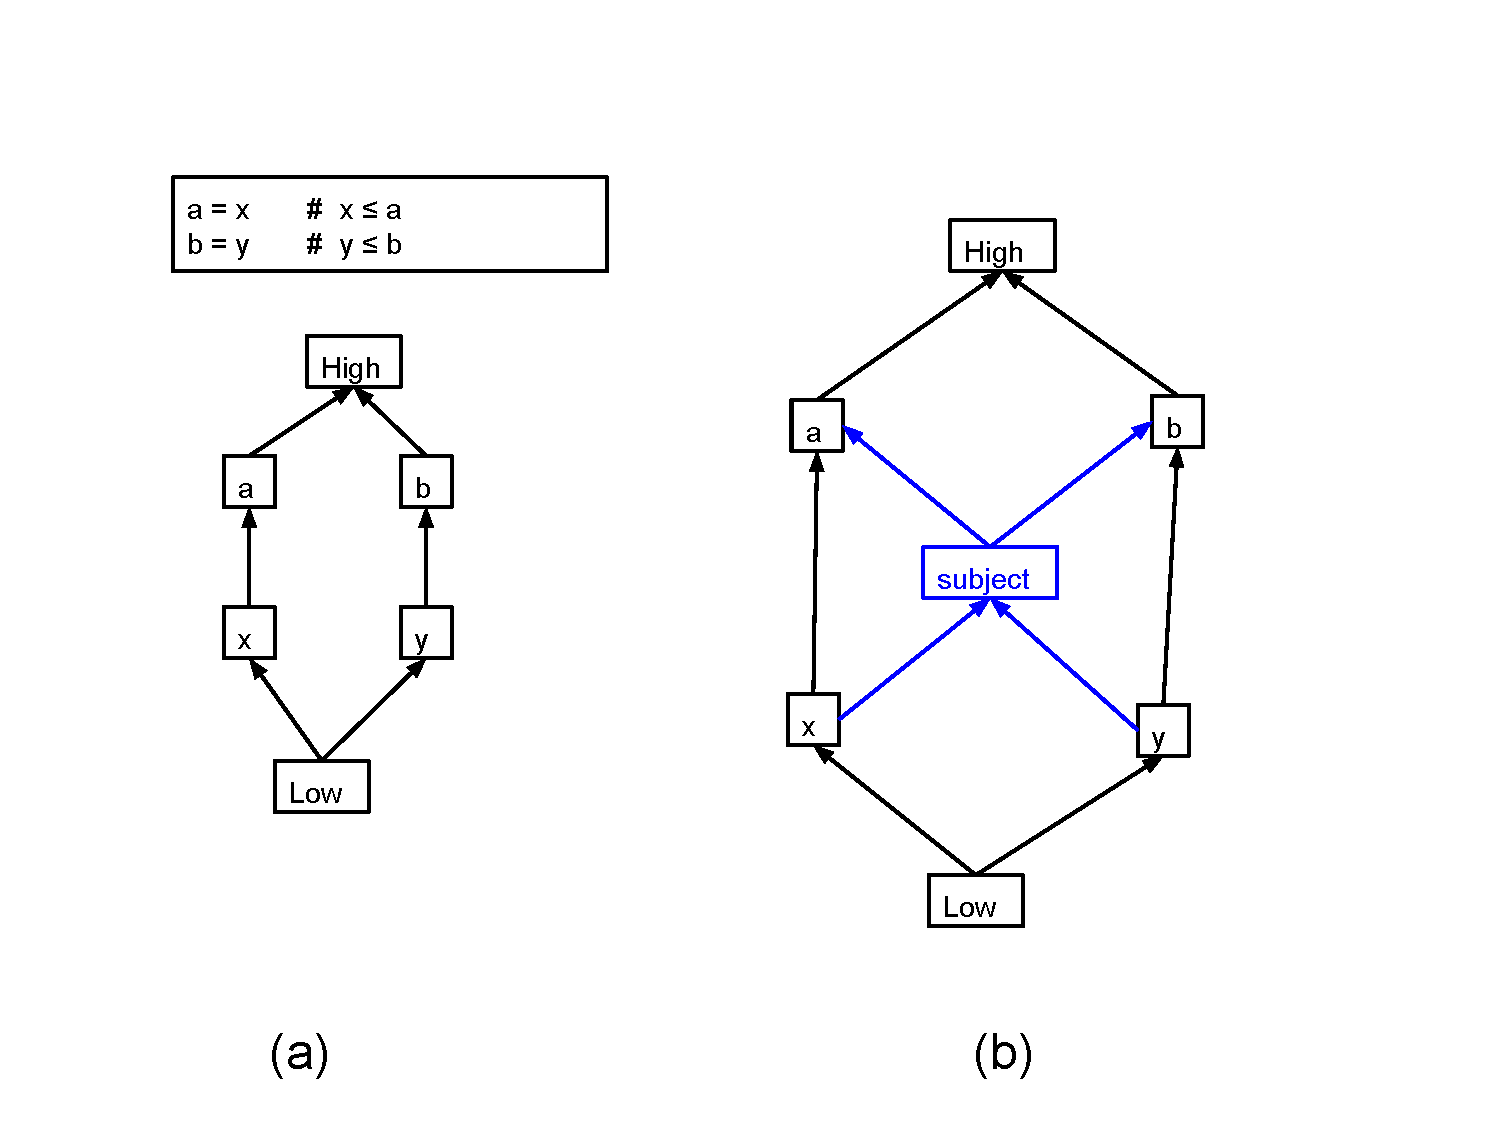
\includegraphics[width=0.8\textwidth]{sub}
			\caption{Lattice for information flow in a =x and y =b,(a)without subject (b) with subject.}
			\label{fig:sublattice}
		\end{figure*}
		In the previous case, we are checking constraints without considering the subject, but now a subject is given as input and we have to check whether given subject has all required permissions to execute all statements without violation of information flow policy. Figure \ref{fig:sublattice} shows that subject needs to read x and write a in order to execute a = x, so it must follow label(x)  $\leqslant_{RWFM}$ label(subject) and label(subject) $\leqslant_{RWFM}$ label(a) to maintain secure information flow. If the subject does not have required permissions for any statement then script returns false otherwise true.     
		}
    \item{\textbf{Check existence of a set of subjects who can execute the program without violating information flow policy. }\\
    	In this case, we need to find a maximal set of those subjects who can pass 2nd case. A naive way to implement it: for each subject run the 2nd test and if it passes, add it in a set; after checking all subjects this set will be desired output. There is an efficient way to do it, any subject can pass 2nd test if and only if it is present in reader set of all objects which lie on the left side of $\leqslant$ operator in constraints and it is  present in writer set of all objects which lie on the right side of $\leqslant$ operator in constraints . So we take the stepwise intersection of all reader sets of objects tht lie in left side of $\leqslant$ operator in constraints and writer sets of all objects that lie on the right side of $\leqslant$ operator in constraints.\\ \textbf{Example:} constraint is given in equation \ref{eqn:cons}\\
    	Conversion of security class of objects into RWFM labels: $x^{(s,R_1,W_1)}$, $y^{(s,R_2,W_2)}$, $z^{(s,R_3,W_3)}$.\\
    	Output of script: $R_1 \cap R_2 \cap W_3$
    	 \begin{equation}\label{eqn:cons}
    	 \dud{x} \oplus \dud{y} \leqslant \dud{z}
    	 \end{equation}
    	       
    }	
\end{enumerate}
%\section{Comparision between Syntatic labels and RWFM label}
%\textbf{Syntatic label(Security class)} : Denning's book \cite{denning} described the use of security class for a multi-level security system in chapter 5, where security class is a pair of two fields (A,C), A: authority label and C: category.     

